\subsection{Vorbereitung}

\begin{enumerate}
\item Zuerst wird ein Zylinderresonator zwischen Mikrofon und Lautsprecher platziert und anschließend mit dem Oszilloskop eine
Resonanz aufgenommen. Dazu wird der Lautsprecher an den einen Kanal des Oszilloskops angeschlossen, das Mikrofon an den
anderen. Von 6,75 kHz an wird die Frequenz nun immer weiter erhöht, bis eine zweite Resonanz gefunden wird.
Es werden Amplitudenspannung, Phasenverschiebung und Frequenz der beiden Resonanzen notiert.

Danach werden mehr und mehr Zylinderresonatoren zwischen Mikrofon und Lautsprecher platziert und die Messung wird
nach jedem neu hinzugefügten Zylinder wiederholt.

\item Im zweiten Teil der Vorbereitung wir das Oszilloskop im xy-Mode betrieben. Dann wird wieder genauso wie im ersten Teil
vorgegangen, wobei das Frequenzspektrum aufgenommen werden soll. Anschließend wird statt eines Oszilloskops ein PC zur
Aufnahme der Spektren genutzt.
\end{enumerate}

\begin{figure}
\centering
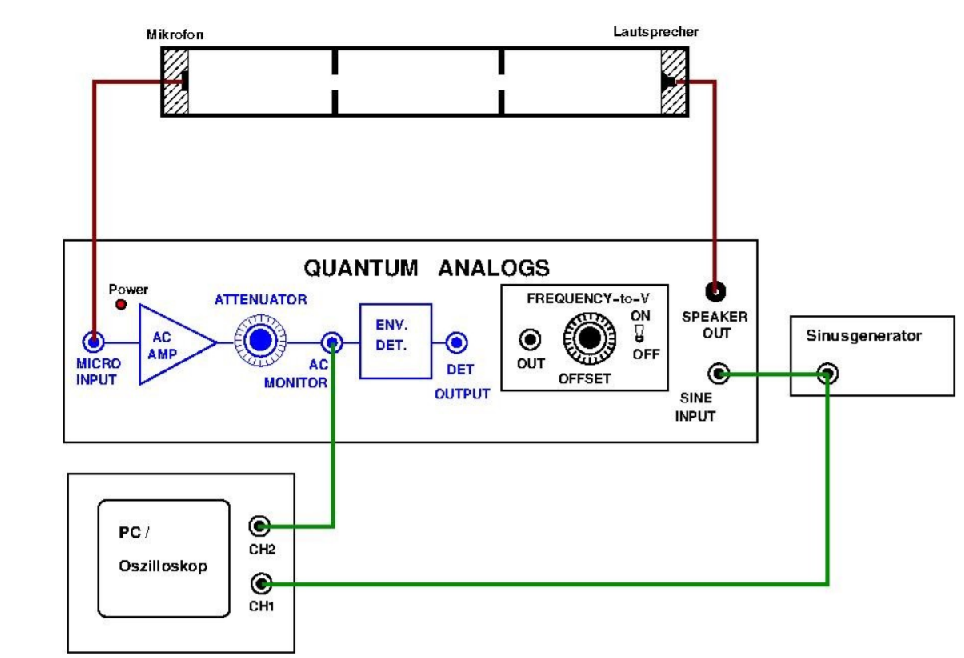
\includegraphics[width=0.6\textwidth]{versuchsaufbau.png}
\caption{Versuchsaufbau für den Versuch "Quantenanalogien". \cite[3]{anleitung}}
\label{fig:versuchsaufbau}
\end{figure}

\subsection{Wasserstoffatom}

In diesem Versuchsteil werden die beiden Kugelhälften mit dem eingebauten Mikrofon und Lautsprecher verwendet. Die beiden
Kugeln werden so aufeinandergesetzt, dass Lautsprecher und Mikrofon sich in einem 180°-Winkel gegenüberliegen. Anschließend
werden folgende Schritte durchgeführt:

\begin{enumerate}
\item Notieren der Resonanzfrequenzen für verschiedene Ordnungen und Beobachtung der Amplituden, Frequenzen und
Phasenverschiebungen (2-Kanal-Oszilloskop, Frequenzbereich 100Hz-10kHz).
\item Für den gleichen Frequenzbereich wird ein Frequenzspektrum mit dem PC aufgenommen.
\item Messung der Druckamplitude als Funktion des Winkels im Bereich 0°-180° für mindestens 3 Resonanzen (10°-Schrittweite).
\item Nacheinander werden Zwischenringe (3mm, 9mm und 3mm+9mm Dicke) zwischen die beiden Kugelhälften eingesetzt, die wieder im
180°-Winkel zueinander stehen und es wird die Aufspaltung der Resonanz bei den Frequenzen 2,1kHz und 2,3kHz vermessen.
\item Erneute Messung der Winkelabhängigkeit wie in Schritt 3 bei den Resonanzfrequenzen 2,1kHz und 2,3kHz. Dieses Mal mit
dem 9mm-Ring zwischen den Kugelhälften.
\end{enumerate}
